\documentclass[14pt, fleqn, xcolor={dvipsnames, table}]{beamer}
\usepackage[T2A]{fontenc}
\usepackage[utf8]{inputenc}
\usepackage[english,russian]{babel}
\usepackage{amssymb,amsfonts,amsmath,mathtext}
\usepackage{cite,enumerate,float,indentfirst}
\usepackage{cancel}
\usepackage{graphicx}
\usepackage{animate}
\usepackage{ulem}

\usepackage{tikz}
% \usepackage{enumitem}
\usetikzlibrary{shadows}

% \usepackage{enumitem}
% \setitemize{label=\usebeamerfont*{itemize item}%
%   \usebeamercolor[fg]{itemize item}
%   \usebeamertemplate{itemize item}}

\graphicspath{{images/}}

\usetheme{Madrid}
\usecolortheme{seahorse}
\renewcommand{\CancelColor}{\color{red}}

\setbeamercolor{footline}{fg=Blue!50}
\setbeamertemplate{footline}{
  \leavevmode%
  \hbox{%
  \begin{beamercolorbox}[wd=.333333\paperwidth,ht=2.25ex,dp=1ex,center]{}%
    И. Кураленок, Н. Поваров, Яндекс
  \end{beamercolorbox}%
  \begin{beamercolorbox}[wd=.333333\paperwidth,ht=2.25ex,dp=1ex,center]{}%
    Санкт-Петербург, 2014
  \end{beamercolorbox}%
  \begin{beamercolorbox}[wd=.333333\paperwidth,ht=2.25ex,dp=1ex,right]{}%
  Стр. \insertframenumber{} из \inserttotalframenumber \hspace*{2ex}
  \end{beamercolorbox}}%
  \vskip0pt%
}
\newcommand\indentdisplays[1]{%
     \everydisplay{\addtolength\displayindent{#1}%
     \addtolength\displaywidth{-#1}}}
\newcommand{\itemi}{\item[\checkmark]}

\newenvironment{mydescription}[1]
  {\begin{list}{}%  
   {\renewcommand\makelabel[1]{\color{blue}##1:\hfill}%
   \settowidth\labelwidth{\makelabel{#1}}%
   \setlength\leftmargin{\labelwidth}
   \addtolength\leftmargin{\labelsep}}}
  {\end{list}}

\title{Ансамбли\\\small{}}
\author[]{\small{%
И.~Куралёнок,
Н.~Поваров}}
\date{}
\begin{document}

\begin{frame}
\maketitle
\small
\begin{center}
\vspace{-60pt}
\normalsize {\color{red}Я}ндекс \\
\vspace{80pt}
\footnotesize СПб, 2014
\end{center}
\end{frame}

\section{Bayes Optimal Classifier}
\begin{frame}{Пример}{Bagginng}
Дмитрий и Владимир выбирают страну, куда поехать на отдых. Их рассуждения: \\
\textit{``Ничего мы не знаем про эту заграницу, давай поспрашиваем у знакомых''} \\
И опросили много народу: Петровича, Славу, Дмитрия, Людвига, Сергея и т.п.\\
~\\
~\\
Надо понять как теперь быть с результатами опроса, и куда же все-таки ехать.
\end{frame}

\begin{frame}{Bayes Optimal Classifier}
Пускай у нас есть несколько способов узнать правду ($H$), тогда лучше всего правда получается так:
{\small
$$
\arg \max_c \sum_t p(c|h_t) p(h_t | X) = \arg \max_c \sum_t p(c|h_t) p(X | h_t) p(h_t) 
$$
}
по большому счету это просто байесово решение в пространстве гипотез. Но есть несколько проблем:
\small
\begin{itemize}
  \item если семейство бесконечно, то мы замучаемся его перебирать;
  \item не всегда классификатор предоставляет $p(c|h_t)$;
  \item как определить prior традиционно не ясно;
  \item получить несмещенный $p(X|h_t)$ нетривиальная задача.
\end{itemize}
\end{frame}

\begin{frame}{Пути построения BOC}
Раз идеальное решение построить не дают, будем сэмплировать (BMA):
\begin{enumerate}
  \item Для каждого сампла:
  \begin{enumerate}
    \item вычислим prior, точность предсказания ($p(1|h,X)$)
    \item из точности предсказания можно получить log likelihood ($log p(X|h)$):
    {\footnotesize$$
    |X| \left(p(1|h,X) \log p(1|h,X) + \left(1 - p(1|h,X)\right) \log \left(1 - p(1|h,X)\right) \right)
    $$}
    \item примем за вес гипотезы $w(h) = p(h) e^{\log p(X|h)}$
  \end{enumerate}
  \item посчитаем результаты с использованием весов.
\end{enumerate}
\end{frame}

\begin{frame}{Сложности BMA}
 ``Для каждого сампла'' --- надо бы конкретезировать да так, чтобы:
\begin{itemize}
\small
  \item чтобы можно было найти $p(c|h_t)$;
  \item работать только там, где высокий $p(h_t | X)$;
  \item иметь дело с однородными гипотезами, чтобы не мучаться с prior;
  \item не концентрироваться вокруг одной точки.
\end{itemize}
А это невозможно без понимания того как устроено семейство решающих функций.
\end{frame}

\section{Random Forest}

\begin{frame}{Какие свойства решающей функции важны?}
\begin{itemize}
  \item Простой способ подбора
  \item Высокая вариативность
  \item Сравнимые результаты
\end{itemize}
Мы знаем такое семейство --- это ж деревья!
\end{frame}

\begin{frame}{Нужные свойства на деревьях}
\small
\textbf{\color{blue}Простой способ подбора:} все просто и быстро параллелится по листьям \\
\textbf{\color{blue}Высокая вариативность:}
\begin{itemize}
  \item менять данные для обучения (например bootstrapping'ом);
  \item разрешать использовать не все факторы, а только некоторые.
\end{itemize}
\textbf{\color{blue}Сравнимые результаты:} мы всегда можем говорить в одних терминах (сколько примеров в листе, куда попала точка, какие параметры распределения etc.)
\end{frame}

\begin{frame}{Random Forest (bagging)}{без фигни}
\textbf{Bagging = bootstrap aggregating}\\
\begin{enumerate}
  \item Сделаем выборку данных $X'$ из $X$ по правилам bootstrap
  \item Построим оптимальное дерево на множестве $X'$
  \item Результат получим равновесным голосованием деревьев
\end{enumerate}
\end{frame}

\begin{frame}{Random Forest как BMA}
Способ обхода решений: ``будем обходить \textit{оптимальные} деревья''. \\
Обход решений мы полагаем эквивалентным обходу выборок из генеральной совокупности одинакового размера.\\
А выборки уже обходим стандартно (за неимением доступа к генеральной совокупности).
\end{frame}

\begin{frame}{Видимые проблемы}
Большинство деревьев будут очень похожи близко от корня, что уменьшает вариативность. \\
$\Rightarrow$ Давайте пожертвуем точностью увеличив вариативность!
\end{frame}

\begin{frame}{Random Forest (bagging)}{оригинальный by Leo Breiman}
\textbf{Bagging = bootstrap aggregating}\\
\begin{enumerate}
  \item Сделаем выборку данных $X'$ из $X$ по правилам bootstrap
  \item Построим оптимальное дерево на этом множестве, используя при разбиении ограниченный набор факторов
  \item Результат получим равновесным голосованием деревьев
\end{enumerate}
\end{frame}

\begin{frame}{Random Forest свойства}{}
\begin{itemize}
  \item Работает!
  \item Много места для шаманства (веса, обрезание, количество, способ голосования, выбор параметров)
  \item На практике легко оверфитнуть на validate, так как результаты сильно зависят от seed
  \item \textbf{Невозможно оверфитнуть через увеличение количества деревьев!}
\end{itemize}
\end{frame}

\section{Boosting}

\begin{frame}{Пример}{Boosting}
\small
Дмитрий и Владимир выбирают страну, куда поехать на отдых. Их рассуждения: \\
\textit{``Ничего мы не знаем про эту заграницу, давай поспрашиваем у знакомых''} \\{\footnotesize
И спросили они Петровича, а он и говорит: ``надо ехать в Европу''! \\
Пошли товарищи к Славе, который был в Болгарии, а он и говорит: ``в Болгарии не очень, но вот на Черном море в целом -- классно'', \\
И пошли они к Людвигу, который отдыхал в Турции, а он и говорит: ...\\
}
~\\
~\\
Надо понять как теперь быть с результатами опроса, и куда же все-таки ехать.
\end{frame}

\begin{frame}{В переводе на русский}
\small
Парни хотят использовать результаты опроса для того, чтобы приближаться к истине с каждым шагом, углубляясь в детали. \\
Было (Bayes Optimal Classifier):
$$
\arg \max_c \sum_t p(c|h_t) p(X | h_t) p(h_t) 
$$
Хотим ввести состояние $S_t$, которое отражает наше текущее понимание предмета:
$$
\arg \max_c \sum_t p(c|h_t) p(X | h_t, S_t) p(h_t|S_t) 
$$
В качестве состояния, например, может выступать текущий ответ по каждой точке $S_{t+1} = \{p(x| H_t)\}_{x \in X}$
\end{frame}

\begin{frame}{Почему это может работать?}
\small
Очевидно, что работает это хуже, чем оригинальный BOC, есть только одна проблема, BOC никак не реализовать, и сравнивать надо с BMA, который сильно зависит от обхода. \\
Всю красоту мы порушили. Будем строить такую решающую функцию:
$$
H_T(x) = e^{\sum_{t=1}^T \alpha_t h_t(x)}
$$
При этом будем ее строить итеративно:
$$\begin{array}{l}
h_{t+1} = \arg \max_{h} p(h | X,H_t) \\
\alpha_{t+1} = \arg \max_{\alpha} p(H_{t+1} | X, h_{t+1}, H_t)
\end{array}$$
\end{frame}

\begin{frame}{Adaptive boosting}{AdaBoost by Y.~Freund, R.~Schapire}
\begin{enumerate}
  \item Введем состояние $S_0 = \{\frac{1}{m}\}_1^m$
  \item Найдем классификатор $h_{t+1}$:
  $$h_{t+1} = \arg \min_h \sum_{i=1}^m s_{ti} I\{y_i \ne h(x_i)\} $$
  \item Если минимум $e_t \ge \frac{1}{2}$, то останавливаемся
  \item $\alpha_{t+1} = \frac{1}{2}\log{1 - e_t \over e_t}$
  \item Обновляем состояние
  $$s_{t+1i} = {s_{ti} e^{-\alpha_{t+1} y_i h_{t+1}(x_i)} \over Z_{t+1}}$$
\end{enumerate}
\end{frame}

\begin{frame}{Свойства AdaBoosting}{}
\begin{itemize}
  \item Прям совсем работает
  \item Ч\textit{о}рная магия
  \item Можно переобучить при определенном количестве итераций
  \item Умеет обучаться после того как все угадал
\end{itemize}
\end{frame}

\begin{frame}{Weak vs. Strong learners}
Как можно видеть из формул, ошибка $h$ большого значения не имеет, важно уметь делать чуть-чуть лучший чем рандом классификатор.\\
Boosting --- это способ сделать из множества \textit{слабых} классификаторов один \textit{сильный}.
\end{frame}

\section{Аналогии}

\begin{frame}{Немного аналогий}{Bagging}
Bagging --- это стрельба по мишени.
\begin{center}
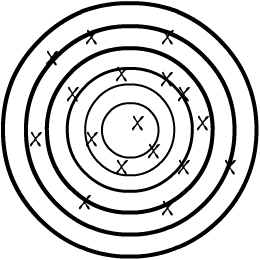
\includegraphics[height=0.4\textheight]{mockup_2.png}
\end{center}
Особо точный лучник порвет мишень! \uncover<2->{$\Rightarrow$ пускай стреляет на звук!} \\
\uncover<3->{Будет смещен в сторону сильных факторов} \uncover<4->{$\Rightarrow$ выдадим ему плохой лук!}
\end{frame}

\begin{frame}{Немного аналогий}{Boosting}
Boosting --- это игра в гольф, когда не важно сколько раз ударил.
\begin{center}
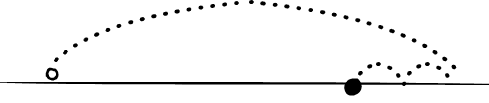
\includegraphics[width=0.8\textwidth]{mockup.png}
\end{center}
Если бить слишком точно, то ансамбль будет слишком короткий. \uncover<2->{$\Rightarrow$ сломаем руки}.\\
\uncover<3->{Получится однообразный} \uncover<4->{$\Rightarrow$ сломаем клюшки}.
\end{frame}

\begin{frame}{Что мы сегодня узнали}
\begin{itemize}
  \item Если есть много классификаторов, то их можно комбинировать
  \item Можно это делать по науке, но железа на всех не хватит
  \item Делая близко к науке (bagging) можно достичь хороших результатов
  \item Если использовать чОрную магию (boosting), то можно получить еще лучше
  \item Узнали что такое weak и strong learner
\end{itemize}
\end{frame}

\section{Bonis track}

\begin{frame}{Немного о ансамблях}
\begin{itemize}
  \item В соревнованиях часто применяются ансамбли, так как всем пофиг насколько сложная получилась модель.
  \item Я ни разу не видел, чтобы выигрывали неравновесные $\alpha$.
\end{itemize}
\end{frame} 

\end{document}
